\begin{figure*}[t]
  \centering
  
\includegraphics[width=.4\linewidth]{figs/legend_methods.pdf}

  \subfloat[Cosmetics ($w=20$)]{%
    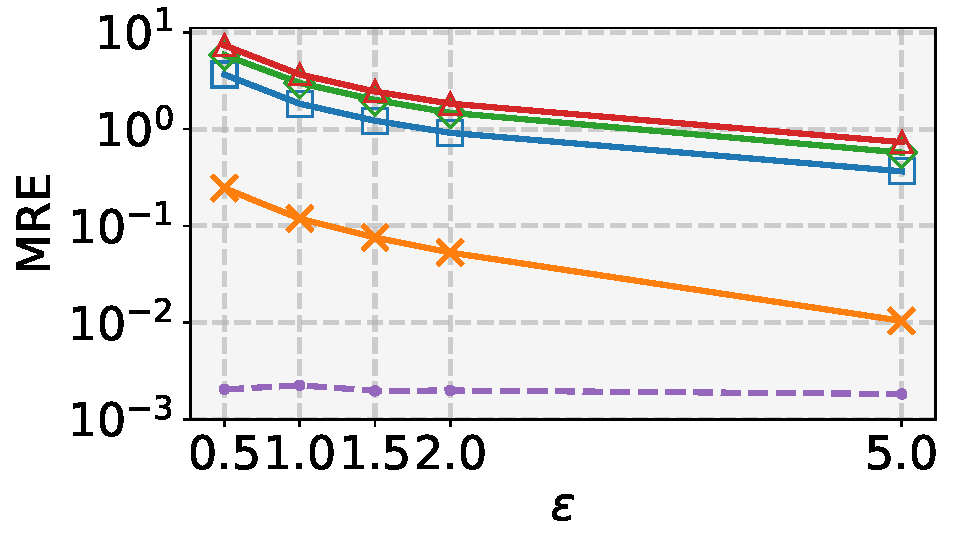
\includegraphics[width=.25\linewidth]{figs/w=20-category.pdf}}
  \subfloat[Cosmetics ($\epsilon=1$)]{%
    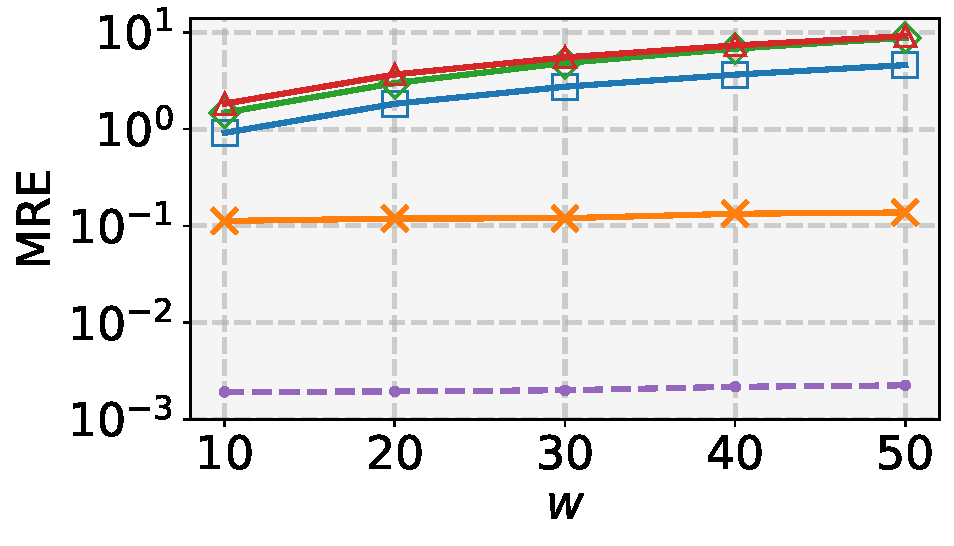
\includegraphics[width=.25\linewidth]{figs/e=1-category.pdf}}
  \subfloat[Cosmetics ($w=20$)]{%
    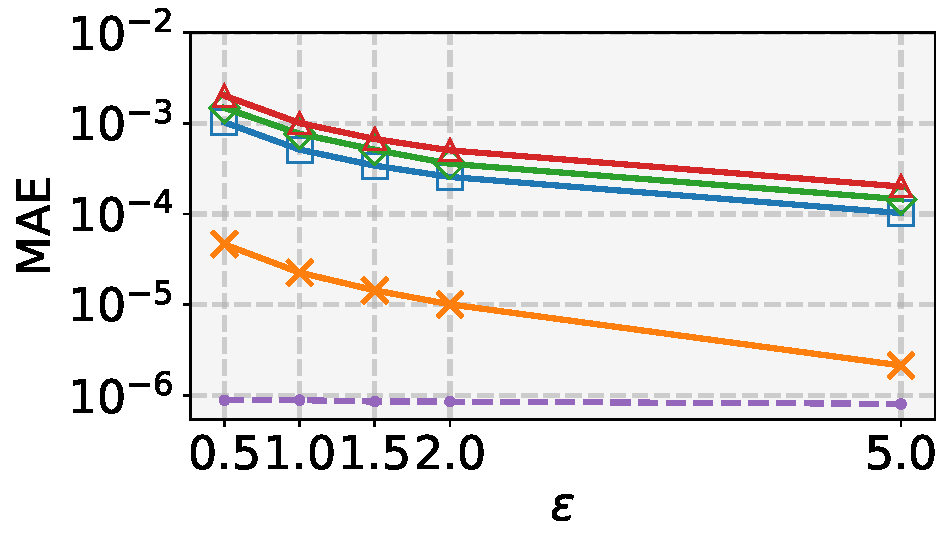
\includegraphics[width=.25\linewidth]{figs/w=20-category-MAE.pdf}}
  \subfloat[Cosmetics ($\epsilon=1$)]{%
    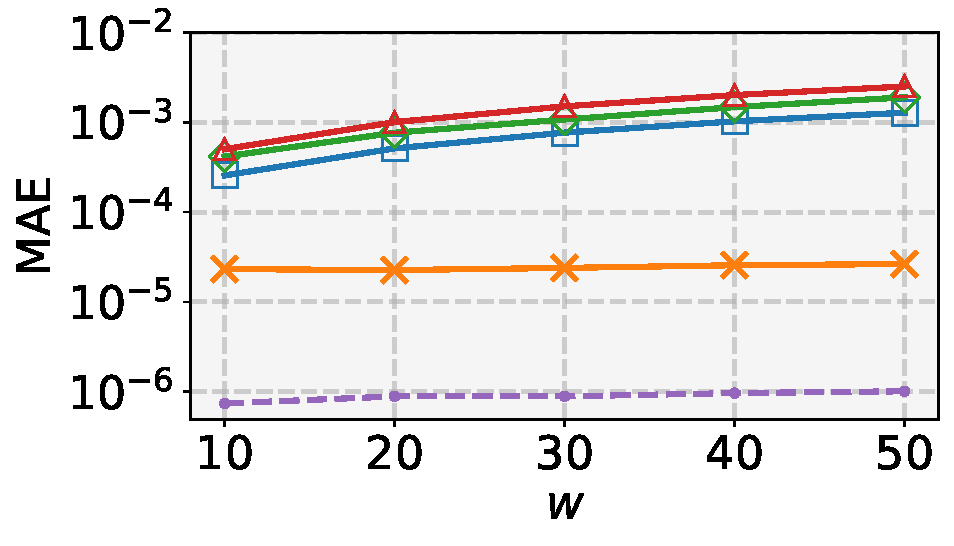
\includegraphics[width=.25\linewidth]{figs/e=1-category-MAE.pdf}}

  \subfloat[Taxi ($w=20$)]{%
    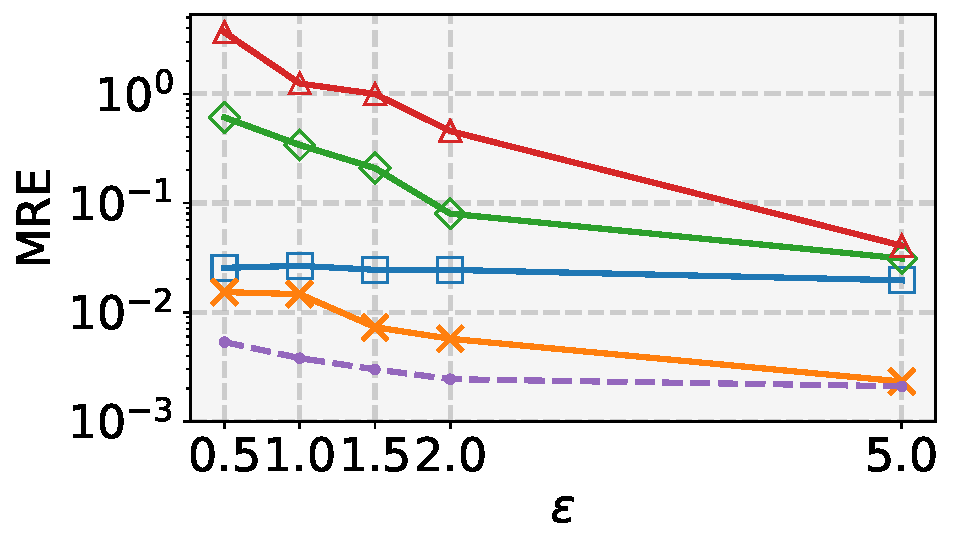
\includegraphics[width=.25\linewidth]{figs/w=20-taxi.pdf}}
  \subfloat[Taxi ($\epsilon=1$)]{%
    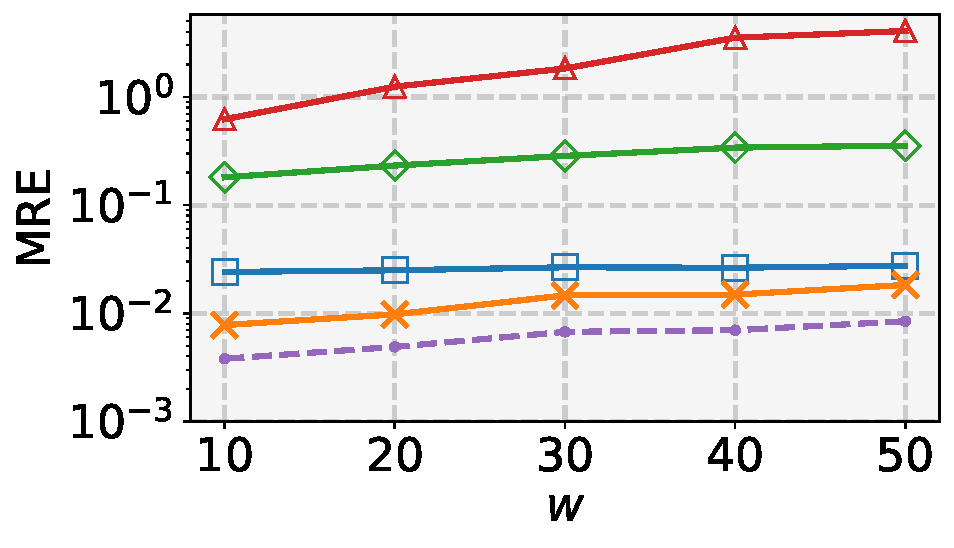
\includegraphics[width=.25\linewidth]{figs/e=1-taxi.pdf}}
  \subfloat[Taxi ($w=20$)]{%
    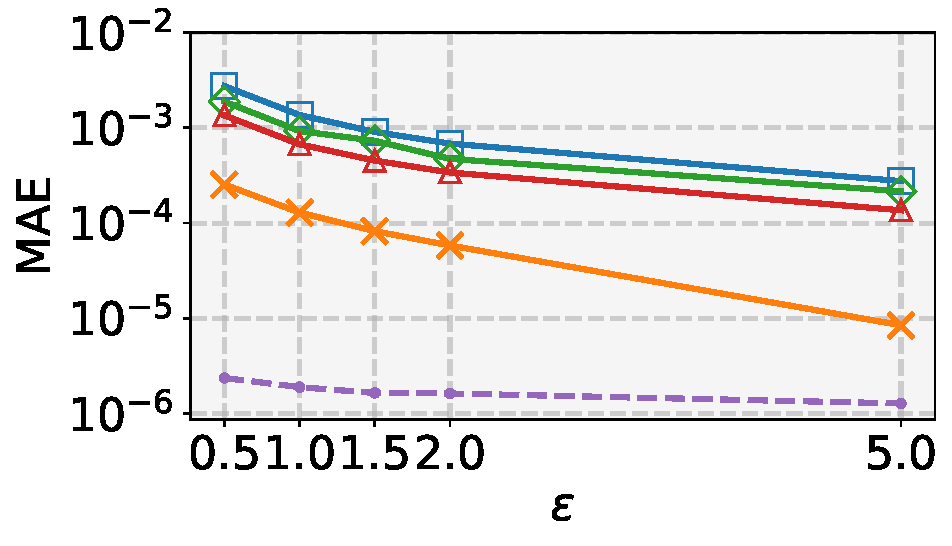
\includegraphics[width=.25\linewidth]{figs/w=20-taxi-MAE.pdf}}
  \subfloat[Taxi ($\epsilon=1$)]{%
    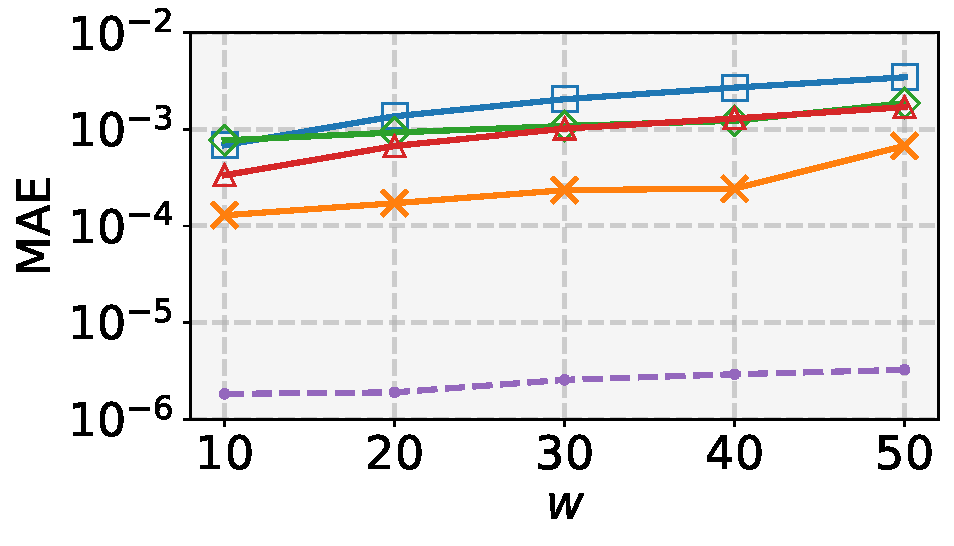
\includegraphics[width=.25\linewidth]{figs/e=1-taxi-MAE.pdf}}

  \subfloat[Loan ($w=20$)]{%
    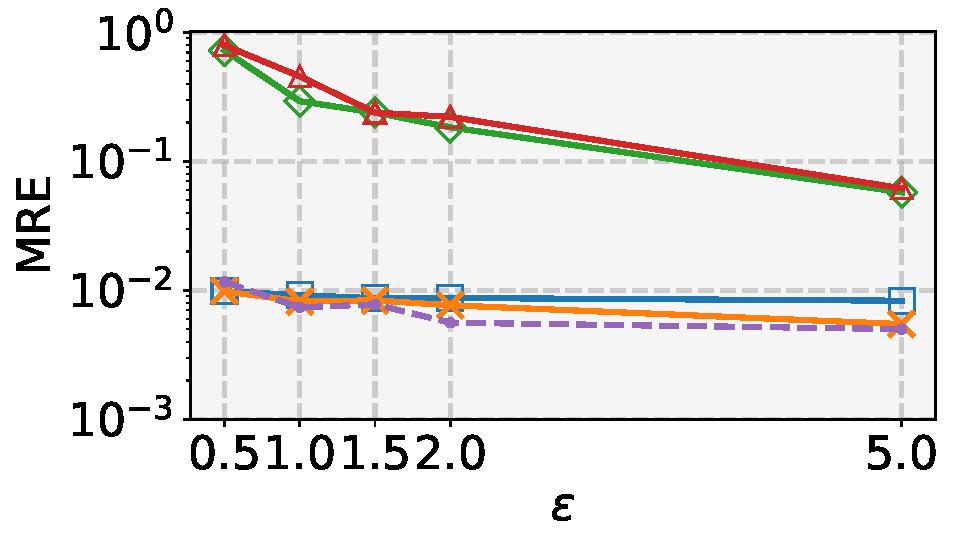
\includegraphics[width=.25\linewidth]{figs/w=20-loan.pdf}}
  \subfloat[Loan ($\epsilon=1$)]{%
    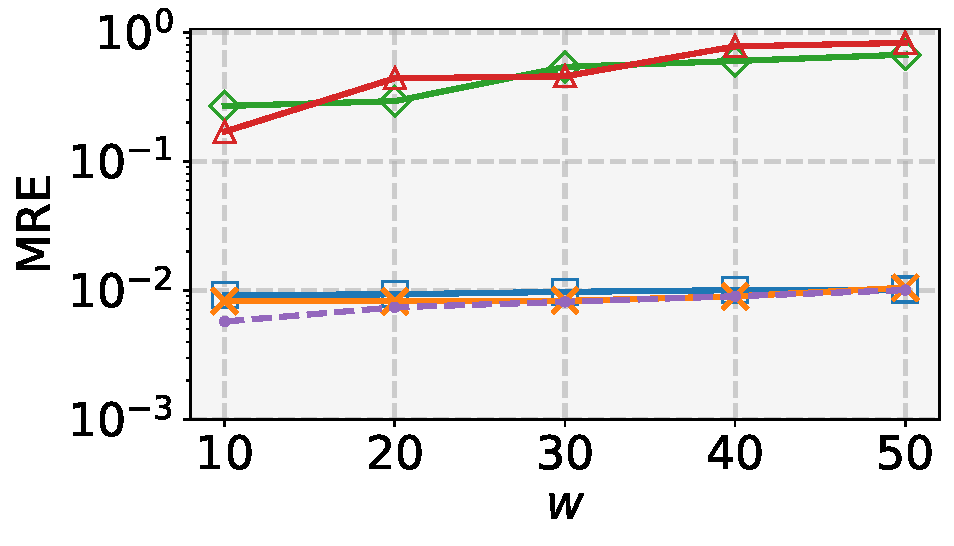
\includegraphics[width=.25\linewidth]{figs/e=1-loan.pdf}}
  \subfloat[Loan ($w=20$)]{%
    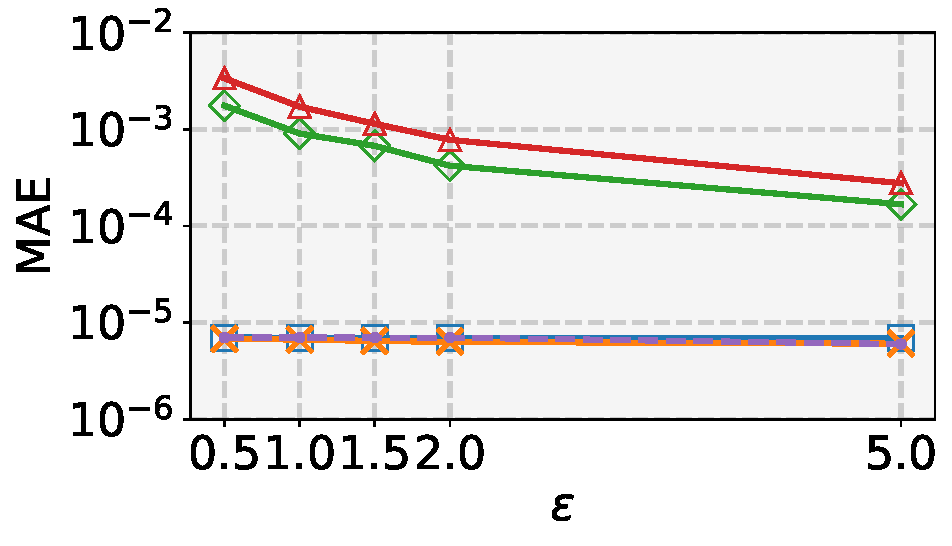
\includegraphics[width=.25\linewidth]{figs/w=20-loan-MAE.pdf}}
  \subfloat[Loan ($\epsilon=1$)]{%
    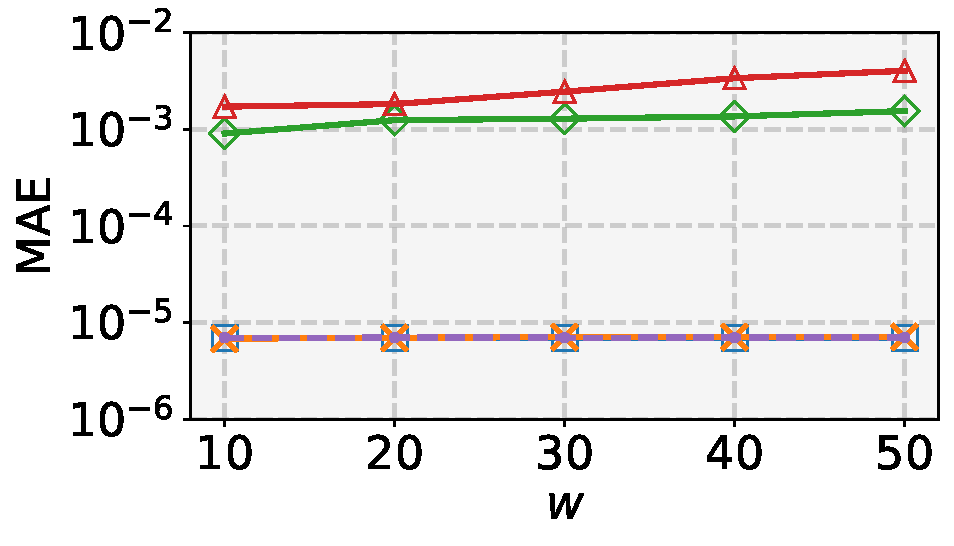
\includegraphics[width=.25\linewidth]{figs/e=1-loan-MAE.pdf}}

  \subfloat[Foursquare ($w=20$)]{%
    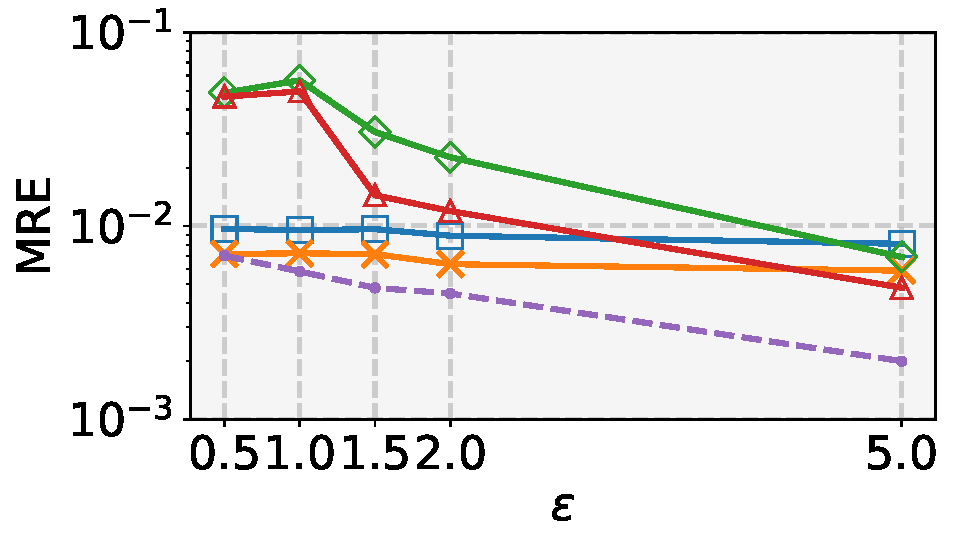
\includegraphics[width=.25\linewidth]{figs/w=20-tist.pdf}}
  \subfloat[Foursquare ($\epsilon=1$)]{%
    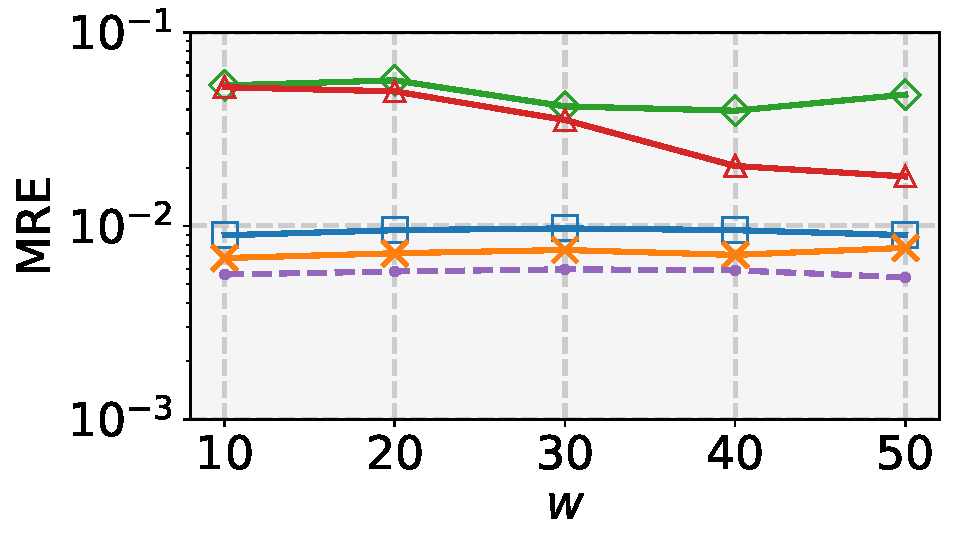
\includegraphics[width=.25\linewidth]{figs/e=1-tist.pdf}}
  \subfloat[Foursquare ($w=20$)]{%
    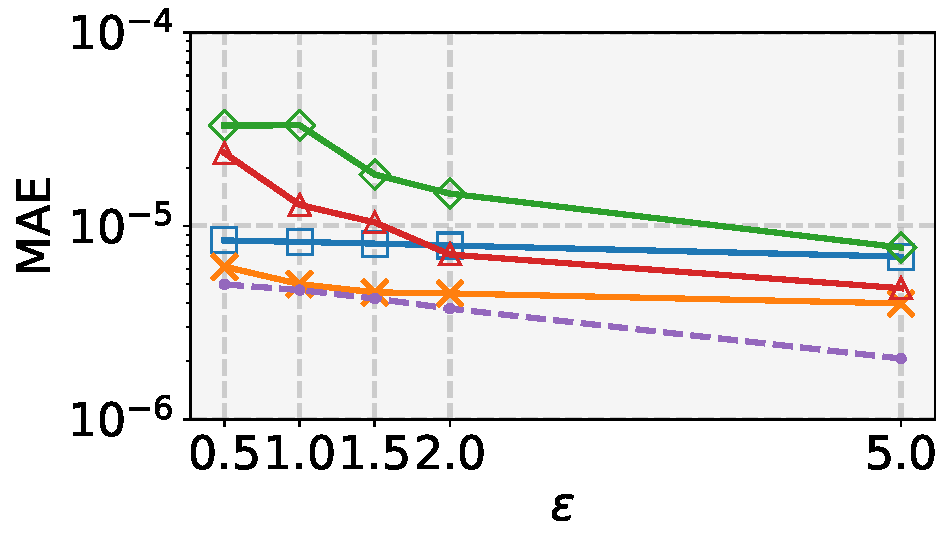
\includegraphics[width=.25\linewidth]{figs/w=20-tist-MAE.pdf}}
  \subfloat[Foursquare ($\epsilon=1$)]{%
    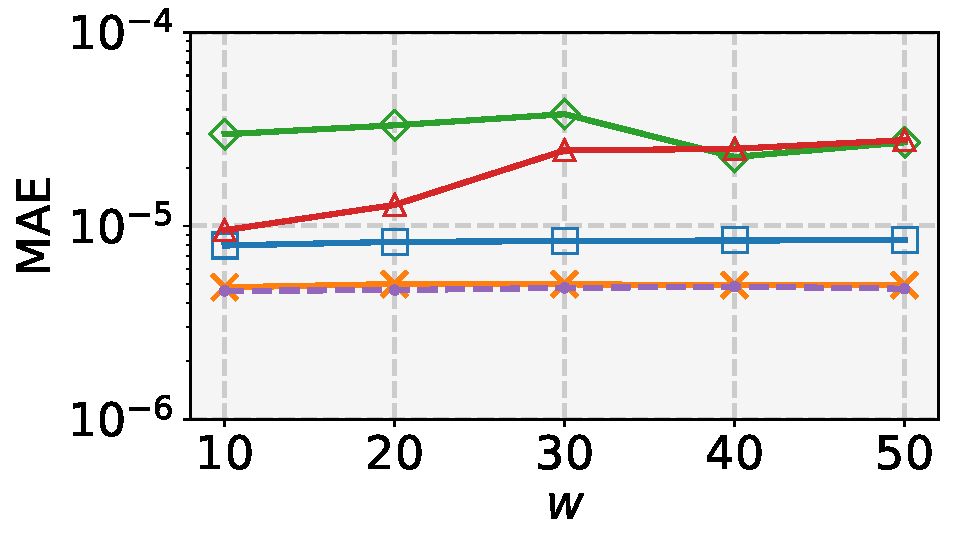
\includegraphics[width=.25\linewidth]{figs/e=1-tist-MAE.pdf}}
  \caption{Counting query evaluation with varying $\epsilon$ and $w$}
  \label{fig:histogram}
  \Description{The figure presents a 4x4 grid of line charts evaluating the performance of counting queries. 
The rows correspond to four datasets: Cosmetics, Taxi, Loan, and Foursquare. 
The columns represent different metrics and varying parameters: the first and second columns show Mean Relative Error (MRE) varying epsilon and window size w, respectively; the third and fourth columns show Mean Absolute Error (MAE) varying epsilon and w. 
Five methods are compared: LBU, LSP, LBD, LBA, and the proposed MTSP-LDP. 
In all 16 subplots, the Y-axis is on a logarithmic scale. 
Visually, the proposed MTSP-LDP method (represented by a purple dashed line) consistently stays at the bottom of all charts, indicating it achieves the lowest error by a significant margin (often orders of magnitude) compared to the four baseline methods across all datasets and parameter settings.}
\end{figure*}
